% Constructed and checked from the problem; not a geometric proof.
\documentclass[tikz,border=8pt]{standalone}
\begin{document}
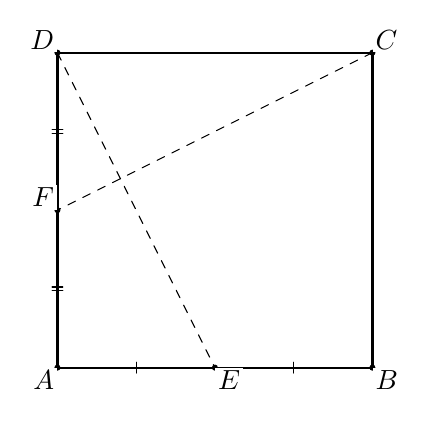
\begin{tikzpicture}[scale=1,line cap=round,line join=round]
\coordinate (p0) at (0,0);
\coordinate (p1) at (4,0);
\coordinate (p2) at (4,4);
\coordinate (p3) at (0,4);
\coordinate (p4) at (2,0);
\coordinate (p5) at (0,2);
\draw[thick] (p0) -- (p1);
\draw[thick] (p1) -- (p2);
\draw[thick] (p2) -- (p3);
\draw[thick] (p3) -- (p0);
\draw[dashed] (p3) -- (p4);
\draw[dashed] (p2) -- (p5);
\draw (1,0.068) -- (1,-0.068);
\draw (3,0.068) -- (3,-0.068);
\draw (-0.068,0.9762) -- (0.068,0.9762);
\draw (-0.068,1.0238) -- (0.068,1.0238);
\draw (-0.068,2.9762) -- (0.068,2.9762);
\draw (-0.068,3.0238) -- (0.068,3.0238);
\fill (p0) circle (1.1pt) node[fill=white,inner sep=1pt,below left] {$A$};
\fill (p1) circle (1.1pt) node[fill=white,inner sep=1pt,below right] {$B$};
\fill (p2) circle (1.1pt) node[fill=white,inner sep=1pt,above right] {$C$};
\fill (p3) circle (1.1pt) node[fill=white,inner sep=1pt,above left] {$D$};
\fill (p4) circle (1.1pt) node[fill=white,inner sep=1pt,below right] {$E$};
\fill (p5) circle (1.1pt) node[fill=white,inner sep=1pt,above left] {$F$};
\end{tikzpicture}
\end{document}
